\documentclass{article}
\usepackage[utf8]{inputenc}
\usepackage[english]{babel}
\usepackage{amssymb,array}
\usepackage{enumitem}
\usepackage[usenames, dvipsnames]{color}
\usepackage[margin=0.5in]{geometry}
\usepackage{amsmath}
\usepackage{graphicx}
\usepackage[superscript,biblabel]{cite}
\usepackage{float}
\usepackage{braket}

\title{\textbf{Template}}
\author{Shane Flynn }
\date{May 2016}

\begin{document}

\maketitle

\section{Introduction}
To start take this file copy and paste everything and make a new project so you can always refer back to this one.
To make your edited pdf appear just click the recompile button!

Latex documents are composed of different "environments" which correlate with different features. 
The beginning of a document lists various packages available to latex, much like any programming language stores external functionality.
Notice at the end of each sentence I start on a new line, this makes editing your file easier when working with a text editor, however it will not change the actual spacing of your document. 

If I skip an entire line it will start a new paragraph as you see here. 
There are various ways of doing things in Latex, and with any good open-source material, the Internet has plenty of answers and examples you can simply copy and paste into your code (no need to reinvent the wheel). 
If I want to put a math symbol in my document I need to make sure I have the math environment at the beginning of my document (as a package).
Here I have the standard packages I currently use, whenever you find a problem, there may already be a solution in terms of a package which you simply need to add to your document. 


For instance, if I skip two lines in my code, I do not get two lines of space in my document, there is a command to make space. 

\bigskip

Now I have a space in between my paragraphs.
Note the commands are given by the programming slash.
\subsection{Share Latex}
As you can guess this tutorial is for using sharelatex, it is the easiest way for a person to learn latex and is very user friendly.
Transitioning from here to a text editor and traditional latex is pretty easy, however some of the compiling is more involved in traditional latex.
So this tutorial will do everything in terms of sharelatex and I have other documents explaining how to work from the terminal. 

\subsubsection{Latex vs Word}
With a working template like this you should be more or less ready to work immediately.
After using latex for a bit of time you will realize how convenient the commands and environments are.
You can use it just like a word document if you want, but its power comes from its control over formatting a document and using a programming-like environment. 
I encourage you to Google anything you want to do in latex and 99.99\% of the time you can just copy and paste an answer into your document.
You will become more efficient and your work will look better with Latex, and submitting a publication becomes a breeze so dive in and enjoy!


\section*{Equations}
These commands are usually intuitive so it is sometimes quicker to just guess to see if a command $\exists$. 
This is our next lesson, most math people like Latex, there are environments for math symbols, as you can see the dollar signs place their contents in a math environment so you can use their symbols. 
Another way to get math is through the equation environment. 

\begin{equation}
k_{eff}=\sqrt{\sum_i{\gamma_i(k_{a,i})^2}}
\end{equation}

Notice in the equation subscripts are simple to make, you need curly brackets to apply to more than one character (ie without them $k_eff$).
If you want text in an equation you need to tell it.
\begin{equation}
\begin{split}
    A = \text{dog}\\
    B = \frac{\partial}{\partial x}\phi^2 = \frac{\partial \phi^2}{\partial x}
\end{split}
\end{equation}

I can also use my "bracket package" to do quantum $\braket{1|e^{-x^2}|2}$, you can also look up different packages and add them to your file just ask stack overflow.
So many people use LaTex that you should never really need to make a new feature honestly. 



So these are some basic equations and any symbol you need will be easy enough to write.

\section{Figures}
The common features that you will need when writing up a paper are symbols and equations, figures, and references.
If you can make all of these things then there is no reason to use a word processor again!
In latex figures and references are stored in a separate file.
You then "call" upon that file to retrieve the figure or reference you want.
In this way you can add in more figures or files, and the document will automatically account for them when you call them.

In sharelatex on the left side by your main text there are a few menus.
Use the upload command to pull a file into our document it will appear in the left toolbar. 
Note that different file types are allowed however .png is the best (I have had issues with other file types and suggest you stay with .png). 
Now that we have the image we want to include it into our document (you use he name of the image without the extension).
\bigskip

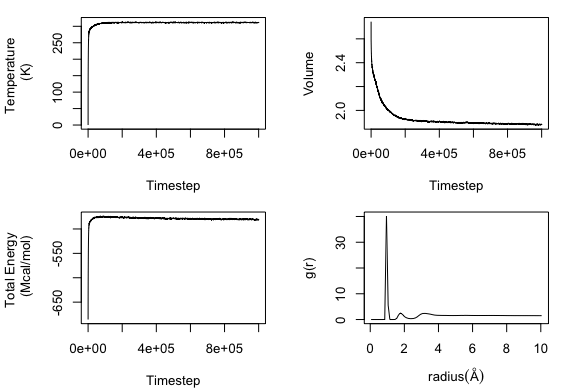
\includegraphics[scale = .5]{equ1_plots}

There are many ways to upload figures, and as you finalize a document you may need to spend some time playing with these for instance here I will adjust the figure manually.

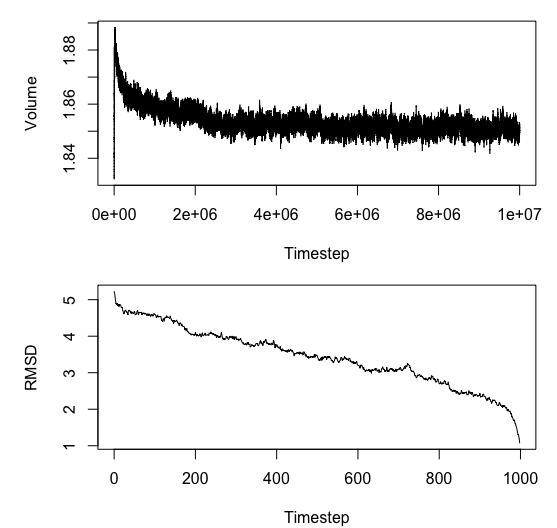
\includegraphics[height=8cm, width=8cm]{equ2_plots}

This is the quickest way to put a figure into a document, but it should not be a surprise that there is a specific environment for doing this.
The figure environment is a better way to put these in and I would only use the include graphics function if you can not get the figure environment to look the way you want. \\
Using the figure environment can be complicated, important things to note are the letters right after begin figure.
This letter specifies where the figure is placed in the file and there are 6 options.
\begin{enumerate}
    \item h = roughly where the code is in the text
    \item t = top of page
    \item b = bottom of page
    \item p = new page
    \item ! = override latex 
    \item H = lace figure exactly where you are in the latex code (you need the float function) \end{enumerate}


\begin{figure}[! h]
    \centering
    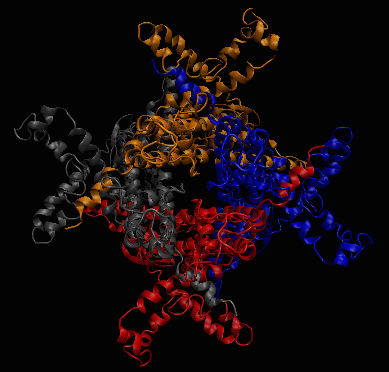
\includegraphics{fig1}
    \caption{Pre-set caption (this makes a caption below, see what happens when you move the caption above include graphics)}
    \label{fig:protein}
\end{figure}

The figure command is better because you can reference it!
It is pretty common to reference a figure later in your report, to do this you add a label to your figure.
You then simply call upon that label for example see figure \ref{fig:protein} on page \pageref{fig:protein}.
Give these labels intuitive names so you can call them easily.


lkd 
\section{References}
For references, Latex has its own method for making bibliographies known as Bibtex (If you go to Google Scholar and click on cite, Bibtex is the first option). 
To make a bibliography go to the left panel and make a new file that has the extension (.bib).
A latex file is (.tex), a bibliography is (.bib) easy enough.
Similar to the figure we will add citations to the bib file and then call upon it in the latex file.
In this way you can add citations whenever and the numbering will always work because you simply call on the file in the text.
So go to google scholar and find the article you wish to cite.
Click on the cite tool and choose bibtex.
Copy and paste this citation into your bib file.
Note the first line on the citation is a flag to call a specific reference, I suggest giving a name that has meaning so calling your reference is easy to do (ie I changed mine to shane and jon).
Now that we have citations we add them with a cite command.
For more control you can use the natbib package other options I prefer the number system I used here\cite{shane}.
To make it this way I included a package that defines citations to be superscripts.
At the end of the document we need to choose how the bibliography is done (there are various styles for citing things)\cite{jon}.
We also need to tell it where are bib file is (do not include the extension). 

\bibliographystyle{unsrt}
\bibliography{references}
\end{document}

